% Provenance (never printed): see sources/outline_sources.md (Year 1: heat sources,
% radiogenic and secular cooling; heat-flow measurement; the steady conductive geotherm
% with heat production; convection against conduction; the lithosphere as a thermal
% boundary layer). Curves from figdata/bachelor-1/geotherms.py; exercise and problem
% values in the Book 3 scratch calculator calc/ch10.py.
\chapter{ميزانية حرارة الأرض}\label{ch:b1:heat-budget}

تحت جبل في جبال الألب اليابانية، في تجويف منجم قديم، ينتظر خزّان يحوي ألف طن من سائل الوميض ومضات ضوء خافتة. أكثرها آتٍ من مضادّات النيوترينو الناتجة عن المفاعلات النووية في البلد المحيط، لكن بعضها يأتي من الأسفل: فاليورانيوم والثوريوم داخل الأرض يطلقان مضادّات نيوترينو عند تفككهما، وهي تعبر الكوكب كله كأنه فارغ. وفي 2135 يومًا من العدّ سجّل الكاشف 841 حدثًا مرشحًا، نُسب منها 106 إلى الأرض نفسها. ومن تلك الحفنة من الومضات قدّر فريقه عام 2011 أن تفكك اليورانيوم والثوريوم يسخّن الأرض بنحو 20 تيراواط. ويفقد الكوكب كله نحو 47. يحسب هذا الفصل الفرق: من أين تأتي حرارة الأرض، وكيف يُقاس الفيض الحراري الخارج منها، وكيف ترتفع الحرارة مع العمق حين تنقلها الموصلية، ولماذا يجب أن يتحرّك \omterm{def:b1:layered-earth:layers}{الوشاح} بالحمل، ولماذا تكون الصفائح الحدّ العلوي البارد لذلك الحمل.

\begin{recall}
يسير \omterm{def:b1:heat-budget:heat-flow}{تدفّق الحرارة} من الساخن إلى البارد؛ والموصلية الحرارية $k$ للصخر تقيس سهولة عبور الحرارة فيه، والانتشارية الحرارية $\kappa = k/(\rho c)$ تقيس سرعة انتشار تغيّر الحرارة (من كتاب الفيزياء للسنة الثانية). وتتفكك الأنوية المشعّة بعمر نصف ثابت (الفيزياء). وترتفع الحرارة مع العمق على امتداد \omterm{def:b1:heat-budget:geotherm}{المنحنى الحراري}، \omterm{def:b1:layered-earth:layers}{والوشاح} يتحرّك بالحمل (الكتاب 2، الصفان 11 و\num{12}). \omterm{def:b1:layered-earth:lithosphere}{والغلاف الصخري} هو \omterm{def:b1:layered-earth:layers}{القشرة} الخارجية القوية للأرض (\cref{ch:b1:layered-earth}).
\end{recall}

\section{من أين تأتي الحرارة}

\begin{definition}[تدفّق الحرارة]\label{def:b1:heat-budget:heat-flow}
\emph{تدفّق الحرارة}\index{تدفّق الحرارة} $q$ عند نقطة من سطح الأرض، أو كثافة التدفّق الحراري السطحي، هو القدرة ذات المنشأ الداخلي التي تعبر السطح هناك، لكل وحدة مساحة، محسوبةً موجبة نحو الخارج. وتُقاس بوحدة \unit{W.m^{-2}}، وعمليًا بوحدة \unit{mW.m^{-2}}. وإذا كُوملت على السطح كله أعطت فقدان الأرض للحرارة $Q = \oint q\,\mathrm dS$.
\end{definition}

قِيس \omterm{def:b1:heat-budget:heat-flow}{تدفّق الحرارة} في عشرات الآلاف من المواقع. وتجميع من \num{38347} قياسًا، نُشر عام 2010، يعطي المتوسطات الآتية، مع عدّ المحيطات والقارات كلٍّ على حدة:
\begin{center}
\small
% ledger: dd10:split, dd10:total
\begin{tabular}{lccc}
\hline
 & المساحة (\unit{m^2}) & فقدان الحرارة (\unit{TW}) & متوسط \omterm{def:b1:heat-budget:heat-flow}{تدفّق الحرارة} (\unit{mW.m^{-2}}) \\
\hline
القارات & \num{2.073e14} & 14.7 & 70.9 \\
المحيطات & \num{3.028e14} & 31.9 & 105.4 \\
الأرض كلها & \num{5.101e14} & 46.7 & 91.6 \\
\hline
\end{tabular}
\end{center}
المجموع، مُقرَّبًا إلى هامش خطئه، هو $Q = \qty[uncertainty-mode=separate]{47 \pm 2}{TW}$. ويخرج ثلثاه عبر قاع المحيط، وهو أحدث وأرقّ من القارات. إنه تدفّق صغير: فالشمس تُرسل نحو \qty{173000}{TW} إلى الأرض، ولا تبلغ الحرارة الداخلية سوى \qty{0.03}{\percent} من ميزانية الطاقة عند السطح. % ledger: nasa:solar-mean
لكنه التدفّق الذي يدفع البراكين والصفائح وبناء الجبال، وله مصدران.

\begin{definition}[إنتاج الحرارة الإشعاعي]\label{def:b1:heat-budget:heat-production}
\emph{إنتاج الحرارة الإشعاعي}\index{إنتاج الحرارة الإشعاعي} $A$ لصخر هو الحرارة المنطلقة لكل وحدة حجم ولكل وحدة زمن من تفكك الأنوية المشعّة التي يحويها، بوحدة \unit{W.m^{-3}}، وعمليًا بوحدة \unit{\micro W.m^{-3}}. وصخر كثافته $\rho$ يحوي كسور كتل $C_i$ من العناصر المولّدة للحرارة، يُطلق كل منها $H_i$ واطًا لكل كيلوغرام من العنصر، له
\[
  A = \rho \sum_i C_i H_i .
\]
\end{definition}

تُنتج أربعة نظائر تقريبًا كل هذه الحرارة، لأنها طويلة العمر، ووفيرة بما يكفي، وغنية بالطاقة: \ce{^{238}U}، و\ce{^{235}U}، و\ce{^{232}Th}، و\ce{^{40}K}. والحرارة لكل كيلوغرام من كل عنصر هي الحرارة لكل كيلوغرام من نظيره المشع مضروبةً في حصة هذا النظير من العنصر (\cref{exo:b1:heat-budget:3}):
\begin{center}
\small
% ledger: dye:isotope-heat, iaea:isotopes
\begin{tabular}{lcccc}
\hline
النظير & نصف العمر (\unit{Gyr}) & \shortstack{الحرارة لكل كغ\\من النظير\\(\unit{W.kg^{-1}})} & \shortstack{حصته من\\العنصر (ذرّات)} & \shortstack{الحرارة لكل كغ\\من العنصر\\(\unit{W.kg^{-1}})} \\
\hline
\ce{^{238}U} & 4.468 & \num{9.513e-5} & \qty{99.274}{\percent} & U: \num{9.85e-5} \\
\ce{^{235}U} & 0.704 & \num{5.685e-4} & \qty{0.720}{\percent} & \\
\ce{^{232}Th} & 14.0 & \num{2.628e-5} & تقريبًا كلّه & Th: \num{2.63e-5} \\
\ce{^{40}K} & 1.248 & \num{2.847e-5} & \qty{0.0117}{\percent} & K: \num{3.40e-9} \\
\hline
\end{tabular}
\end{center}
يُطلق البوتاسيوم حرارةً لكل كيلوغرام أقل بثلاثين ألف مرة من اليورانيوم، لكنه عنصر رئيسي في صخور كثيرة، يُعدّ بالنسبة المئوية حيث يُعدّ اليورانيوم والثوريوم بالجزء في المليون. وأغنى الصخور بالعناصر الثلاثة هي الغرانيتات وأقاربها؛ وأفقرها بيريدوتيتات \omterm{def:b1:layered-earth:layers}{الوشاح}. وتعطي مجموعة من 2188 تحليلًا هذه الوسائط، بوحدة \unit{\micro
W.m^{-3}}:
\begin{center}
\small
% ledger: vila:heat-production
\begin{tabular}{lclclc}
\hline
الرايوليت & 2.55 & الصخور الطينية & 1.44 & الغابرو & 0.35 \\
الغرانيت & 2.43 & الحجر الرملي & 0.82 & البازلت & 0.21 \\
الغرانوديوريت & 1.88 & الصخور الكربوناتية & 0.42 & الصخور فوق القاعدية & 0.11 \\
\hline
\end{tabular}
\end{center}
الانتشار داخل كل مجموعة واسع: فربع الغرانيتات ينتج أقل من \qty{1.74}{\micro W.m^{-3}}، وربعها أكثر من \qty{3.23}{\micro W.m^{-3}}. وتغتني \omterm{def:b1:layered-earth:layers}{القشرة} القارية بهذه العناصر، وتفقرها \omterm{def:b1:layered-earth:layers}{القشرة} المحيطية \omterm{def:b1:layered-earth:layers}{والوشاح}؛ لكن \omterm{def:b1:layered-earth:layers}{الوشاح} كبير جدًا بحيث يظل يحوي حصة كبيرة من منابع حرارة الكوكب.

\begin{definition}[التبريد الدهري]\label{def:b1:heat-budget:secular-cooling}
\emph{التبريد الدهري}\index{التبريد الدهري} هو الجزء من فقدان الأرض للحرارة الذي يأتي من انخفاض بطيء في حرارة باطنها، أي \omterm{def:b1:layered-earth:layers}{الوشاح} واللب: إطلاق الحرارة المخزّنة منذ تكوّن الكوكب، بمعدل $-\sum_j M_j c_j\,\mathrm dT_j/\mathrm dt$ للخزانات ذات الكتلة $M_j$ والحرارة النوعية $c_j$ والحرارة المتوسطة $T_j$.
\end{definition}

يعطي حفظ الطاقة ميزانية الأرض كلها: فالحرارة المفقودة عند السطح هي الإنتاج الإشعاعي مضافًا إليه \omterm{def:b1:heat-budget:secular-cooling}{التبريد الدهري}،
\[
  Q = H_{\text{إشعاعي}} + Q_{\text{تبريد}} .
\]
تقيس النيوترينوات الأرضية جزءًا من الحد الأول: فنتيجة 2011، التي جمعت كاشفين، تنسب \qty{20}{TW} إلى اليورانيوم والثوريوم، و\ce{^{40}K}، الذي لا تُكتشف مضاداته بذلك الشكل لضعفها، معروف بأنه يضيف نحو \qty{4}{TW}.
% ledger: kamland:2011
إذن نحو نصف فقدان الحرارة إشعاعي، والنصف الآخر، نحو \qty{23}{TW}، هو \omterm{def:b1:heat-budget:secular-cooling}{التبريد الدهري}. وجزء من ذلك التبريد من اللب: إذ تُقدَّر الحرارة العابرة \omterm{def:b1:layered-earth:discontinuity}{لحدّ اللب–الوشاح} ب\qtyrange{5}{15}{TW}. وهذه الأرقام غير مؤكدة: فالقياس نفسه يحمل خطأً نحو \qty{9}{TW}، ونتائج النيوترينوات الأرضية حتى الآن لا تحصر الجزء الإشعاعي إلا في \qtyrange{15}{41}{TW}، بينما تتراوح نماذج الأرض من أنواع مختلفة بين \qtyrange{14}{46}{TW}. والمجموع المقيس عند السطح هو أعرف حدود الميزانية (الشكل أدناه).
% ledger: dye:radiogenic

\begin{omfigure}
\begin{tikzpicture}[x=0.24cm, y=1cm, font=\small]
% ledger: dd10:split, kamland:2011, dye:radiogenic
% losses
\fill[blue!22] (0,1.6) rectangle (31.9,2.3);
\fill[brown!35] (31.9,1.6) rectangle (46.6,2.3);
\draw (0,1.6) rectangle (46.6,2.3);
\draw (31.9,1.6) -- (31.9,2.3);
\node at (15.95,1.95) {المحيطات 31.9};
\node at (39.25,1.95) {القارات 14.7};
\node[anchor=east, align=right, font=\small] at (-0.5,1.95) {مفقودة عند\\السطح};
% sources
\fill[orange!35] (0,0) rectangle (20,0.7);
\fill[yellow!45] (20,0) rectangle (24,0.7);
\fill[red!18] (24,0) rectangle (46.7,0.7);
\draw (0,0) rectangle (46.7,0.7);
\draw (20,0) -- (20,0.7) (24,0) -- (24,0.7);
\node at (10,0.35) {اليورانيوم والثوريوم 20};
\node at (22,0.35) {البوتاسيوم 4};
\node at (35.35,0.35) {التبريد الدهري $\approx 23$};
\node[anchor=east, align=right] at (-0.5,0.35) {المصادر};
% core part of secular cooling (range)
\draw[red!60!black, very thick] (24,-0.25) -- (29,-0.25);
\draw[red!60!black, thick, densely dashed] (29,-0.25) -- (39,-0.25);
\draw[red!60!black] (24,-0.15) -- (24,-0.35) (39,-0.15) -- (39,-0.35);
\node[anchor=north, font=\scriptsize, red!60!black] at (31.5,-0.3) {الحرارة العابرة لحدّ اللب–الوشاح، \qtyrange{5}{15}{TW}};
% radiogenic range
\draw[|-|, orange!70!black, thick] (15,1.0) -- (41,1.0);
\node[anchor=south, font=\scriptsize, orange!70!black] at (28,1.02) {مدى التقديرات الإشعاعية، \qtyrange{15}{41}{TW}};
% axis
\draw[->] (0,-1.05) -- (50,-1.05) node[right] {TW};
\foreach \x in {0,10,20,30,40} {\draw (\x,-1.0) -- (\x,-1.1) node[below, font=\scriptsize] {\x};}
\end{tikzpicture}
\par\smallskip{\small ميزانية حرارة الأرض. أعلى: الحرارة المفقودة عبر قاع المحيط والقارات، \qty[uncertainty-mode=separate]{47 \pm 2}{TW} في المجموع. أسفل: مصادرها، مع الجزء الإشعاعي لليورانيوم والثوريوم كما قاسته النيوترينوات الأرضية، والجزء الخاص بالبوتاسيوم مقدَّرًا؛ والباقي بالفرق هو \omterm{def:b1:heat-budget:secular-cooling}{التبريد الدهري}، الذي يوفّر اللب جزءًا منه غير معروف جيدًا. ويبيّن الشريط البرتقالي مدى الجزء الإشعاعي الذي تسمح به قياسات النيوترينوات الأرضية.}
\label{fig:b1:heat-budget:budget}
\end{omfigure}

كانت الحرارة الإشعاعية أكبر في الماضي، لأن النظائر كانت أوفر: ف\ce{^{235}U} و\ce{^{40}K}، وهما قصيرا العمر، أسهما آنذاك أكثر بكثير (الكتاب 2، الصف 12). وآلة الحرارة في الأرض تبطؤ ببطء، من الجهتين.

\section{قياس تدفّق الحرارة}

لا يُقاس \omterm{def:b1:heat-budget:heat-flow}{تدفّق الحرارة} مباشرةً: بل يُحسب من تدرّج الحرارة والموصلية.

\begin{proposition}[قانون فورييه]\label{prop:b1:heat-budget:fourier}
في وسط موصليته الحرارية $k$، تنتقل الحرارة على طول تدرّج الحرارة بمعدل لكل وحدة مساحة يتناسب معه. مع $z$ العمق محسوبًا موجبًا نحو الأسفل، و$q$ محسوبًا موجبًا نحو الأعلى،
\[
  q = k\,\frac{\mathrm dT}{\mathrm dz} .
\]
\end{proposition}
\admitted

يُثبَت القانون في مجلد الفيزياء للسنة الثانية. وتوصل معظم الصخور الحرارة بمعدل \qtyrange{1.5}{3}{W.m^{-1}.K^{-1}} تحت \qty{200}{\celsius}، وأقل حين تكون ساخنة؛ وتعطي نماذج \omterm{def:b1:heat-budget:heat-flow}{تدفّق الحرارة} القارّي \omterm{def:b1:layered-earth:layers}{للقشرة} العليا الغرانيتية نحو \qty{2.7}{W.m^{-1}.K^{-1}}؛
% ledger: delaney:conductivity, roy:granitic-k
وتدرّج قدره \qty{25}{K.km^{-1}} فيها يعني تدفّقًا حراريًا نحو \qty{70}{mW.m^{-2}}.

حين تختلف الموصلية للصخور التي يعبرها ثقب حفر، يتغيّر التدرّج من صخرة إلى التي تليها، لكن \omterm{def:b1:heat-budget:heat-flow}{تدفّق الحرارة} لا يتغيّر ما دام لا تُنتَج حرارة ولا تُخزَّن بينها. وتحوّل المبرهنة التالية ذلك إلى اختبار.

\begin{proposition}[مخطط بولارد]\label{prop:b1:heat-budget:bullard}
ليكن $R(z) = \int_0^z \mathrm d\zeta/k(\zeta)$ المقاومة الحرارية، لكل وحدة مساحة، للصخور بين السطح والعمق $z$، بوحدة \unit{m^2.K.W^{-1}}. إذا كان \omterm{def:b1:heat-budget:heat-flow}{تدفّق الحرارة} $q$ هو نفسه عند كل عمق في ثقب الحفر، فإن الحرارة دالة خطية في المقاومة الحرارية: $T(z) = T_0 + q\,R(z)$.
\end{proposition}

\begin{proof}
بقانون فورييه، $\mathrm dT/\mathrm dz = q/k(z)$. وبالتكامل من $0$ إلى $z$ مع ثبات $q$، $T(z) - T_0 = q\int_0^z \mathrm d\zeta/k(\zeta) = q\,R(z)$.
\end{proof}

\begin{method}[تدفّق الحرارة من ثقب حفر]\label{met:b1:heat-budget:borehole}
\begin{enumerate}
  \item سجّل الحرارة على طول الثقب بعد الحفر بزمن طويل، حين يكون اضطراب سائل الحفر قد زال، واستبعد أقرب عشرات الأمتار، فهي تتبع الفصول.
  \item قِس موصلية عينات اللب لكل صخرة يعبرها الثقب في المختبر، واحسب المقاومة الحرارية $R(z)$ عند كل عمق مسجَّل.
  \item ارسم $T$ بدلالة $R$: ميل الخط المستقيم هو \omterm{def:b1:heat-budget:heat-flow}{تدفّق الحرارة}. ويكشف الانحناء عن ماء يجري عبر الصخور، أو تغيّرًا قديمًا في حرارة السطح، أو خطأً في موصلية.
  \item صحّح، حيث يلزم، لأثر التضاريس، التي تحني الخطوط المتساوية الحرارة تحت التلال والوديان، ولأثر الاحترار البطيء منذ آخر عصر جليدي، الذي ما زال يُخلّ بالكيلومتر العلوي تقريبًا.
\end{enumerate}
\end{method}

في البحر لا حاجة إلى ثقب. فحرارة قاع المحيط العميق ثابتة جدًا، حتى إن بضعة أمتار من الرواسب اللينة تحمل التدرّج التوازني. وتُلقى من السفينة قضيبٌ فولاذي يحمل صفًّا من مجسّات الحرارة، ويُدفع إلى الرواسب بثقل ثقيل (الشكل أدناه)؛ فتسجّل المجسّات التدرّج، وتعطي نبضة حرارية تُرسل على طول القضيب موصلية الرواسب في موضعها.
لقاع المحيط مصيدة واحدة: فعلى \omterm{def:b1:layered-earth:layers}{القشرة} الفتية يدور ماء البحر خلال البازلت المتشقّق، ويحمل معه جزءًا كبيرًا من الحرارة بالانتقال بالحمل، فيقصر \omterm{def:b1:heat-budget:heat-flow}{تدفّق الحرارة} الموصلي المقاس كثيرًا عن الفقدان الحقيقي. ولذلك يُحسب الفقدان عبر أحدث قاع المحيط بنموذج التبريد من \cref{sec:b1:heat-budget:boundary-layer}، المعايَر على \omterm{def:b1:layered-earth:layers}{قشرة} قديمة توقّف فيها الدوران: وهذا الجزء المحسوب، \qty{23.1}{TW}، يبلغ نحو نصف المجموع العالمي. % ledger: dd10:young-ocean

\begin{omfigure}
\begin{tikzpicture}[font=\scriptsize, x=1cm, y=1cm]
% --- left: borehole on land ---
\fill[brown!12] (0,0) rectangle (3.2,-1.6);
\fill[red!10] (0,-1.6) rectangle (3.2,-4.2);
\draw[thick] (0,0) -- (3.2,0);
\node[anchor=west] at (0.05,-0.8) {الصخر الطيني، $k$ منخفضة};
\node[anchor=west] at (0.05,-2.9) {الغرانيت، $k$ مرتفعة};
\draw[black!60] (0,-1.6) -- (3.2,-1.6);
\draw[very thick] (2.5,0.3) -- (2.5,-4.0);
\draw[gray] (2.5,0.6) -- (2.5,0.3);
\foreach \y in {-0.6,-1.2,-1.8,-2.4,-3.0,-3.6} {\fill[red!70!black] (2.5,\y) circle (1.6pt);}
\node[anchor=south] at (2.5,0.6) {سجلّ الحرارة};
% inset T(z)
\draw[->] (3.7,0) -- (5.6,0) node[right] {$T$};
\draw[->] (3.7,0) -- (3.7,-4.2) node[below] {$z$};
\draw[thick, red!70!black] (3.9,-0.1) -- (4.9,-1.6) -- (5.4,-4.0);
\node[anchor=west, align=left] at (4.9,-1.0) {شديد الانحدار في\\الصخر الطيني};
\node[anchor=west, align=left] at (5.25,-3.0) {أقل انحدارًا في\\الغرانيت};
\node[anchor=north] at (2.6,-4.45) {(أ) ثقب حفر: $q = k\,\mathrm dT/\mathrm dz$ في كل صخرة};
% --- right: probe at sea ---
\begin{scope}[xshift=8.6cm]
\fill[blue!8] (0,0) rectangle (5.4,-2.6);
\draw[blue!50, thick] (0,0) .. controls (0.6,0.08) and (1.2,-0.08) .. (1.8,0)
  .. controls (2.4,0.08) and (3.0,-0.08) .. (3.6,0) .. controls (4.2,0.08) and (4.8,-0.08) .. (5.4,0);
\fill[gray!60] (1.6,0.02) -- (3.0,0.02) -- (2.8,0.3) -- (1.8,0.3) -- cycle;
\node[anchor=south] at (2.3,0.32) {السفينة};
\draw[gray] (2.4,0.02) -- (2.4,-2.75);
\fill[brown!25] (0,-2.6) rectangle (5.4,-4.2);
\draw (0,-2.6) -- (5.4,-2.6);
\node[anchor=west] at (3.0,-3.0) {رواسب لينة};
\node[anchor=west] at (3.0,-3.4) {(بضعة أمتار)};
\fill[black!70] (2.2,-2.75) rectangle (2.6,-3.0);
\draw[very thick] (2.4,-3.0) -- (2.4,-4.0);
\foreach \y in {-3.2,-3.45,-3.7,-3.95} {\fill[red!70!black] (2.4,\y) circle (1.6pt);}
\node[anchor=east, align=right] at (2.1,-2.85) {ثقل};
\node[anchor=east, align=right] at (2.25,-3.55) {قضيب مع\\مجسّات};
\node[anchor=west] at (0.1,-1.3) {ماء عميق، حرارة ثابتة};
\node[anchor=north] at (2.7,-4.45) {(ب) في البحر: مسبار يُدفع في الرواسب};
\end{scope}
\end{tikzpicture}
{\small قياس \omterm{def:b1:heat-budget:heat-flow}{تدفّق الحرارة} (تخطيطي، غير مرسوم بمقياس). (أ) على اليابسة تُسجَّل الحرارة على طول ثقب حفر بعدما عادت إلى التوازن، وتُقاس موصلية كل صخرة على اللبّ: التدرّج أشدّ حيث تكون الموصلية أدنى، \omterm{def:b1:heat-budget:heat-flow}{وتدفّق الحرارة}، حاصل ضربهما، واحد. (ب) في البحر يُدفع قضيب بمجسّات بضعة أمتار في رواسب قاع المحيط.}
\label{fig:b1:heat-budget:measure}
\end{omfigure}

\begin{inthefield}[تدفّق الحرارة في البحر]
\begin{minipage}[t]{0.55\linewidth}\vspace{0pt}
على سفينة بحثية، يكون مسبار \omterm{def:b1:heat-budget:heat-flow}{تدفّق الحرارة} قضيبًا ثقيلًا معلّقًا من رافعة المؤخرة. يُنزل بكابل السفينة حتى يصبح فوق قاع البحر مباشرةً، ثم يُترك: فيدفعه الثقل إلى الرواسب، ويجلس الطاقم على السطح بينما تستقر المجسّات على حرارة الطين، ثم يُسحب القضيب وتنتقل السفينة إلى المحطة التالية على مسافة قصيرة. وخط من هذه المحطات عبر منحدر حيد يعطي تناقص \omterm{def:b1:heat-budget:heat-flow}{تدفّق الحرارة} مع عمر القاع، والتشتت بين المحطات المتجاورة يبيّن أين يجري الماء عبر \omterm{def:b1:layered-earth:layers}{القشرة} التي تحتها.
\end{minipage}\hfill
\begin{minipage}[t]{0.42\linewidth}\vspace{0pt}
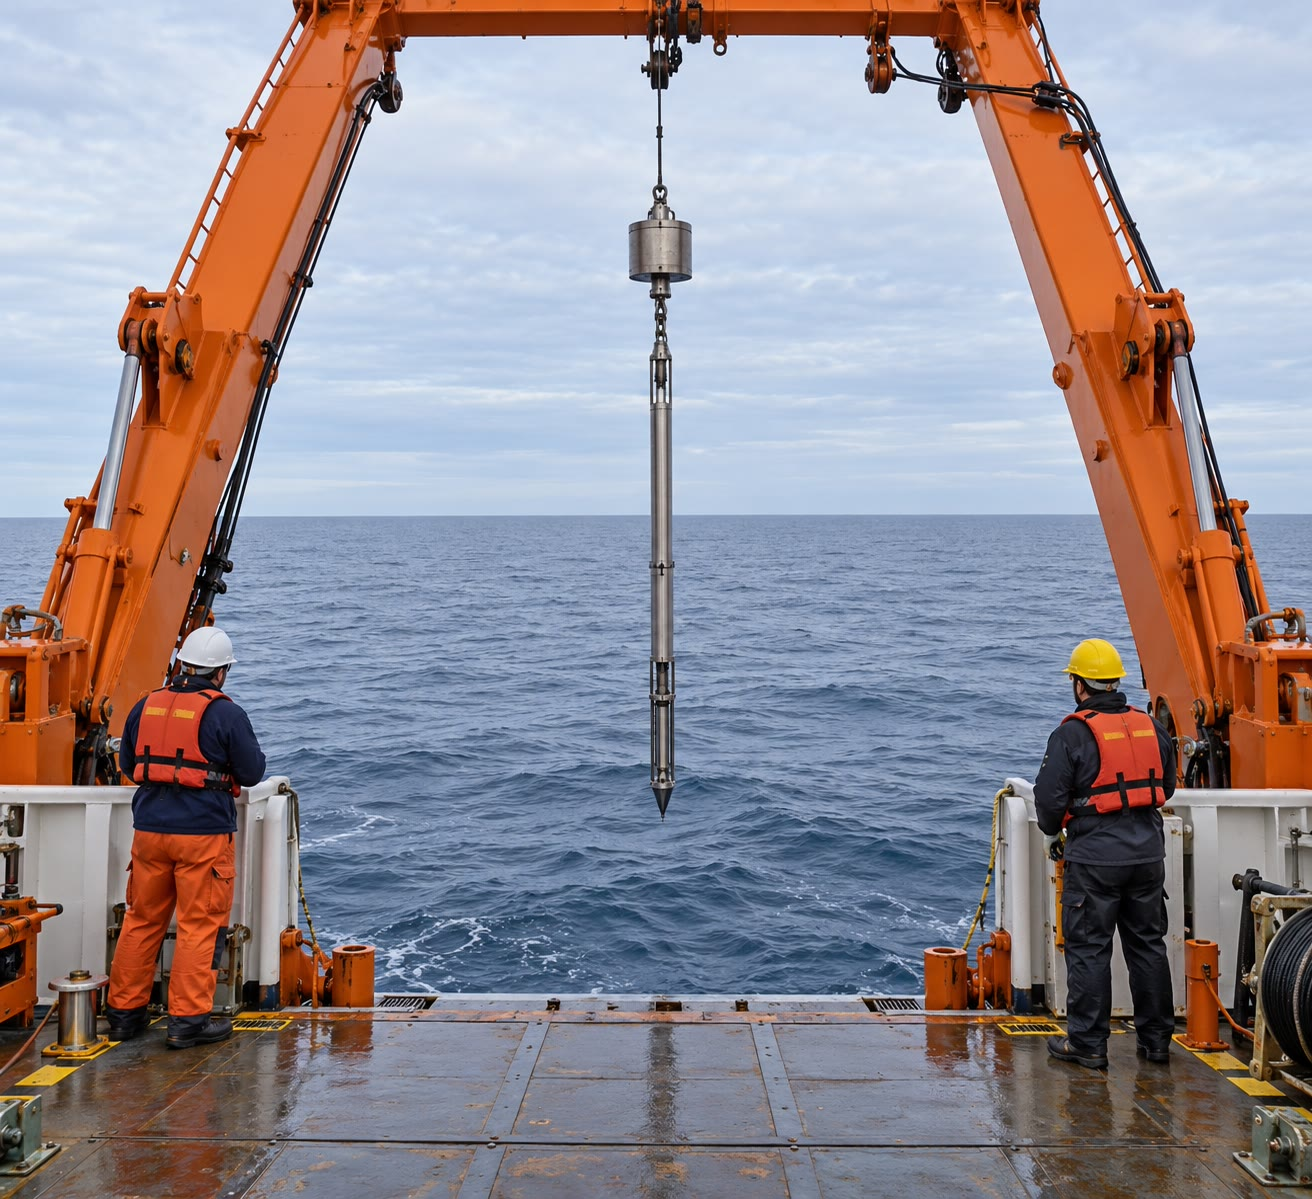
\includegraphics[width=\linewidth]{images/book3/ai/b1-heatflow-probe.jpg}

{\scriptsize مسبار تدفّق حراري معلّق من رافعة مؤخرة سفينة بحثية (رسم توضيحي مُولَّد بالذكاء الاصطناعي).}
\end{minipage}
\end{inthefield}

\section{المنحنى الحراري الموصل المستقر}

\begin{definition}[المنحنى الحراري]\label{def:b1:heat-budget:geotherm}
\emph{المنحنى الحراري}\index{المنحنى الحراري} تحت نقطة من السطح هو الحرارة دالةً للعمق هناك، $T(z)$. وهو منحنٍ حراري موصل مستقر حين لا يتغيّر مع الزمن، وتُحمل الحرارة على امتداده بالموصلية وحدها.
\end{definition}

ضمن \omterm{def:b1:layered-earth:lithosphere}{الغلاف الصخري}، بعيدًا عن البراكين النشطة ودوران الماء، تُحمل الحرارة بالموصلية، وعلى مقياس ملايين السنين يكون \omterm{def:b1:heat-budget:geotherm}{المنحنى الحراري} مستقرًا. وشكله يتبع إذن من موازنة الطاقة.

\begin{theorem}[التوصيل المستقر مع إنتاج الحرارة]\label{thm:b1:heat-budget:balance}
على امتداد منحنى حراري موصل مستقر، في وسط موصليته المنتظمة $k$ وإنتاجه الحراري $A(z)$ دون تدفّق أفقي للحرارة،
\[
  \frac{\mathrm dq}{\mathrm dz} = -A(z), \qquad\text{أي}\qquad
  k\,\frac{\mathrm d^2T}{\mathrm dz^2} = -A(z).
\]
\end{theorem}

\begin{proof}
لتكن شريحة أفقية مساحتها $S$ بين العمقين $z$ و$z +
\mathrm dz$. تدخل الحرارة من قاعدتها بمعدل $q(z + \mathrm dz)\,S$، وتخرج من قمتها بمعدل $q(z)\,S$، وتُنتج داخلها بمعدل $A(z)\,S\,\mathrm dz$. وفي الحالة المستقرة لا تُخزَّن حرارة، ف$q(z)\,S = q(z + \mathrm dz)\,S + A(z)\,S\,\mathrm dz$، أي $\mathrm dq/\mathrm dz = -A$. وبقانون فورييه $q = k\,\mathrm dT/\mathrm dz$، ومع $k$ منتظمة، $k\,T'' = -A$.
\end{proof}

وعند القراءة من السطح نحو الأسفل، ينخفض \omterm{def:b1:heat-budget:heat-flow}{تدفّق الحرارة} مع العمق بمقدار الحرارة المنتجة فوق كل مستوى: فما يعبر السطح هو الحرارة القادمة من الأسفل مضافًا إليها كل الحرارة المنتجة في الطريق. وتعطي توزيعان ل$A$ صيغًا مغلقة.

\begin{proposition}[طبقة إشعاعية منتظمة]\label{prop:b1:heat-budget:uniform}
لتكن الحرارة المنتجة $A$ من السطح حتى العمق $h$ وصفرًا تحته، وليكن السطح عند الحرارة $T_0$، \omterm{def:b1:heat-budget:heat-flow}{وتدفّق الحرارة} السطحي $q_0$. عندئذٍ، من أجل $0 \le z \le h$،
\[
  q(z) = q_0 - A z, \qquad T(z) = T_0 + \frac{q_0 z}{k} - \frac{A z^2}{2k},
\]
وتحت $h$ يكون \omterm{def:b1:heat-budget:heat-flow}{تدفّق الحرارة} منتظمًا، $q_m = q_0 - A h$، \omterm{def:b1:heat-budget:geotherm}{والمنحنى الحراري} خطًا مستقيمًا ميله $q_m/k$.
\end{proposition}

\begin{proof}
نكامل $\mathrm dq/\mathrm dz = -A$ من $0$ مع $q(0) = q_0$: $q = q_0 -
Az$. ثم $\mathrm dT/\mathrm dz = (q_0 - Az)/k$؛ وبالتكامل مع $T(0) = T_0$ يُحصل على القطع المكافئ. وتحت $h$، $\mathrm dq/\mathrm dz = 0$ ويحتفظ $q$ بقيمته عند $h$.
\end{proof}

\begin{theorem}[إنتاج الحرارة الأسّي والعلاقة الخطية لتدفّق الحرارة]
\label{thm:b1:heat-budget:exponential}
ليتناقص إنتاج الحرارة مع العمق وفق $A(z) = A_0 e^{-z/D}$، ويتجه \omterm{def:b1:heat-budget:heat-flow}{تدفّق الحرارة} إلى $q_m$ عند العمق الكبير، ولتكن حرارة السطح $T_0$. عندئذٍ
\[
  q(z) = q_m + A_0 D\,e^{-z/D}, \qquad
  T(z) = T_0 + \frac{q_m z}{k} + \frac{A_0 D^2}{k}\bigl(1 - e^{-z/D}\bigr),
\]
\omterm{def:b1:heat-budget:heat-flow}{وتدفّق الحرارة} السطحي هو
\[
  q_0 = q_m + A_0 D .
\]
\end{theorem}

\begin{proof}
من \cref{thm:b1:heat-budget:balance}، $\mathrm dq/\mathrm dz =
-A_0e^{-z/D}$، إذن $q(z) = A_0 D e^{-z/D} + C$؛ وحين $z \to \infty$، $q \to C$، ومنه $C = q_m$. وعند $z = 0$، $q_0 = q_m + A_0 D$. ثم $\mathrm dT/\mathrm dz =
q/k = q_m/k + (A_0D/k)\,e^{-z/D}$، وبالتكامل من $0$ مع $T(0) = T_0$،
$T = T_0 + q_m z/k + (A_0 D^2/k)(1 - e^{-z/D})$.
\end{proof}

السطر الأخير تنبؤ يمكن اختباره عند السطح. فتتشارك أجسام الغرانيت المتطفّلة في منطقة واحدة \omterm{def:b1:heat-budget:heat-flow}{تدفّق الحرارة} العميق نفسه $q_m$، وإذا اختلفت فقط في غناها باليورانيوم والثوريوم والبوتاسيوم، فلها المقياس $D$ نفسه؛ وعندئذٍ ينبغي أن يكون \omterm{def:b1:heat-budget:heat-flow}{تدفّق الحرارة} المقاس فوق كل جسم دالة خطية لإنتاج الحرارة المقاس في صخوره، ميلها $D$ طول، ومقطعها $q_m$، أي \omterm{def:b1:heat-budget:heat-flow}{تدفّق الحرارة} المخفَّض القادم من أسفل الطبقة المشعّة. ولاحظ فرانسيس بيرش أول خط من هذا النوع، ونُشر عام 1968، وفي العام نفسه حُدّدت ثلاث مقاطعات بخطوطها:
\begin{center}
\small
% ledger: roy:provinces, roy:linear-relation
\begin{tabular}{lcc}
\hline
المقاطعة & المقطع $q_m$ (\unit{mW.m^{-2}}) & الميل $D$ (\unit{km}) \\
\hline
شرق الولايات المتحدة & 33 & 7.5 \\
منطقة الحوض والسلاسل & 59 & 9.4 \\
سييرا نيفادا & 17 & 10 \\
\hline
\end{tabular}
\end{center}
القيم المقطعية، المنشورة ك\num{0.8} و\num{1.4} و$0.4\times\qty{e-6}{cal.cm^{-2}.s^{-1}}$، تُحوَّل ب$\qty{1}{\micro cal.cm^{-2}.s^{-1}} = \qty{41.84}{mW.m^{-2}}$ (\cref{exo:b1:heat-budget:4}). وتتغيّر الميول قليلًا، من 7 إلى \qty{10}{km}؛ أما \omterm{def:b1:heat-budget:heat-flow}{تدفّق الحرارة} المخفَّض فيتغيّر كثيرًا، وخرائطه تبيّن أين يكون \omterm{def:b1:layered-earth:layers}{الوشاح} تحته ساخنًا، كما تحت \omterm{def:b1:layered-earth:layers}{القشرة} المتمدّدة في منطقة الحوض والسلاسل. ويعطي الطبقة المنتظمة من \cref{prop:b1:heat-budget:uniform} أيضًا خطًا مستقيمًا، ميله $h$: فالنموذجان يطابقان المعطيات، لكن النموذج الأسّي وحده يبقى خطًا مستقيمًا بالميل نفسه حين تُنحت الأجسام المتطفّلة إلى أعماق مختلفة (\cref{exo:b1:heat-budget:10})، ولهذا يُفضَّل.

\begin{omfigure}
\begin{tikzpicture}
\begin{axis}[omdepth, width=0.82\linewidth, height=8.6cm, xmin=0, xmax=1800, ymin=0, ymax=250, axis x line=top, axis y line=left, axis line style={-}, clip=true,
  xlabel={\foreignlanguage{arabic}{الحرارة \babelsublr{(\unit{\degreeCelsius})}}}, ylabel={\foreignlanguage{arabic}{العمق \babelsublr{(km)}}},
  tick label style={font=\scriptsize}, label style={font=\small},
  legend style={font=\scriptsize, at={(0.02,0.02)}, anchor=south west, draw=none, fill=white, fill opacity=0.85, text opacity=1},
  legend cell align=left]
\addplot[very thick, black!45] table[x=T, y=depth] {figdata/out/bachelor-1-geotherms-adiabat.dat};
\addlegendentry{منحنى الوشاح الأديباتي}
\addplot[very thick, red!75!black] table[x=T45, y=depth] {figdata/out/bachelor-1-geotherms-continental.dat};
\addlegendentry{$q_0 = \qty{70}{mW.m^{-2}}$}
\addplot[very thick, orange!80!black] table[x=T30, y=depth] {figdata/out/bachelor-1-geotherms-continental.dat};
\addlegendentry{$q_0 = \qty{55}{mW.m^{-2}}$}
\addplot[very thick, green!45!black] table[x=T15, y=depth] {figdata/out/bachelor-1-geotherms-continental.dat};
\addlegendentry{$q_0 = \qty{40}{mW.m^{-2}}$}
\addplot[thick, blue!70!black, densely dashdotted] table[x=T, y=depth] {figdata/out/bachelor-1-geotherms-oceanic.dat};
\addlegendentry{قاع محيط عمره \qty{60}{Myr}}
\addplot[thin, dashed, red!75!black, forget plot] table[x=Tc45, y=depth] {figdata/out/bachelor-1-geotherms-continental.dat};
\addplot[thin, dashed, orange!80!black, forget plot] table[x=Tc30, y=depth] {figdata/out/bachelor-1-geotherms-continental.dat};
\addplot[thin, dashed, green!45!black, forget plot] table[x=Tc15, y=depth] {figdata/out/bachelor-1-geotherms-continental.dat};
\draw[densely dotted, black!60] (axis cs:0,35) -- (axis cs:1800,35);
\node[font=\scriptsize, anchor=south east] at (axis cs:1790,35) {موهو، \qty{35}{km}};
\fill (axis cs:1384.0,70.8) circle (1.6pt);
\fill (axis cs:1403.2,107.8) circle (1.6pt);
\fill (axis cs:1459.7,224.9) circle (1.6pt);
\node[font=\scriptsize, anchor=west] at (axis cs:1420,66) {\qty{71}{km}};
\node[font=\scriptsize, anchor=west] at (axis cs:1440,104) {\qty{108}{km}};
\node[font=\scriptsize, anchor=west] at (axis cs:1495,222) {\qty{225}{km}};
\end{axis}
\end{tikzpicture}

\par\smallskip{\small المنحنيات الحرارية الموصلة المستقرة لقارة ذات إنتاج حراري $A_0 = \qty{2.5}{\micro W.m^{-3}}$ يتناقص عبر $D = \qty{10}{km}$، و$k = \qty{2.5}{W.m^{-1}.K^{-1}}$، لثلاثة تدفّقات حرارة سطحية (تدفّقات مخفّضة 15 و\num{30} و\qty{45}{mW.m^{-2}}). يتبع كل منها منحناه الموصل (منقّطًا بعد ذلك) نحو \omterm{def:b1:heat-budget:adiabat}{منحنى الوشاح الأديباتي}، الذي يلتقي به عند النقطة: قاعدة الغلاف الحراري الصخري. ومنحنى قاع المحيط هو منحنى نصف فضاء مبرَّد لمدة \qty{60}{Myr}. والتوصيلية المنتظمة تبسيط.}
\label{fig:b1:heat-budget:geotherms}
\end{omfigure}

\begin{method}[درجة الحرارة على عمق تحت جسم متطفّل]\label{met:b1:heat-budget:moho}
\begin{enumerate}
  \item قِس \omterm{def:b1:heat-budget:heat-flow}{تدفّق الحرارة} السطحي $q_0$ فوق الجسم (طريقة الثقب)، وإنتاجه الحراري $A_0$ من محتواه من اليورانيوم والثوريوم والبوتاسيوم.
  \item من خط المقاطعة، أو بقيمة ل$D$ نحو \qty{10}{km}، احسب $q_m = q_0 - A_0 D$.
  \item طبّق \cref{thm:b1:heat-budget:exponential}. تحت بضعة أضعاف من $D$ يصبح $e^{-z/D}$ مهملًا، ويكون \omterm{def:b1:heat-budget:geotherm}{المنحنى الحراري} الخط المستقيم $T_0 + A_0D^2/k + q_m z/k$: فالطبقة المشعّة رفعت كل حرارة عميقة بمقدار $A_0D^2/k$.
\end{enumerate}
\end{method}

في الشكل تتراوح حرارة \omterm{def:b1:layered-earth:discontinuity}{موهو} من نحو \qty{320}{\degreeCelsius} لأدنى تدفّق حرارة إلى أكثر من \qty{700}{\degreeCelsius} لأعلاه: \omterm{def:b1:heat-budget:heat-flow}{فتدفّق الحرارة} عند السطح يحمل قراءة مباشرة لحرارة \omterm{def:b1:layered-earth:layers}{القشرة} العميقة، التي تحكم متانتها (\cref{ch:b1:stress-strain-rheology}).

\section{التوصيل ضد الحمل}

التوصيل بطيء. ويتبيّن مدى بطئه من معادلة الحرارة، التي تشتقّها كتب الفيزياء من قانون فورييه ومن موازنة \cref{thm:b1:heat-budget:balance} مع إضافة التخزين: في بُعد واحد، دون إنتاج حراري، $\partial T/\partial t = \kappa\,\partial^2 T/\partial z^2$.

\begin{proposition}[زمن التوصيل المميّز]\label{prop:b1:heat-budget:timescale}
يمتد تغيّر حرارة مفروض عند حدّ جسم موصل على مسافة $L$ في زمن من رتبة
\[
  \tau = \frac{L^2}{\kappa} .
\]
\end{proposition}

\begin{proof}
لنكتب $z = L z^*$، و$t = \tau t^*$، مع $z^*$ و$t^*$ بلا أبعاد. تصبح معادلة الحرارة $\partial T/\partial t^* = (\kappa\tau/L^2)\,\partial^2
T/\partial z^{*2}$. وحلولها تتغيّر على مقياس $z^* \sim 1$ حين $t^* \sim 1$ فقط إذا كان المعامل من رتبة الواحد، أي إذا كان $\tau \sim L^2/\kappa$.
\end{proof}

للصخور $\kappa \approx \qty{e-6}{m^2.s^{-1}}$. ويصل التغيّر اليومي للحرارة إلى بضعة عشرات من السنتيمترات داخل الأرض، والسنوي إلى بضعة أمتار، والاحترار منذ آخر عصر جليدي إلى كيلومتر تقريبًا. وعبر \omterm{def:b1:layered-earth:lithosphere}{غلاف صخري} سمكه \qty{100}{km}، $\tau = \qty{e16}{s}$، نحو \qty{300}{Myr}. وعبر \omterm{def:b1:layered-earth:layers}{الوشاح}، البالغ سمكه \qty{2900}{km}، $\tau = \qty{8.4e18}{s}$، أي \qty{270}{Gyr}: ستين ضعف عمر الأرض، \qty{4.54}{Gyr}. % ledger: england:kelvin, usgs:age-earth
ولم يكن التوصيل وحده ليوصل حرارة \omterm{def:b1:layered-earth:layers}{الوشاح} العميق إلى قرب السطح في أي مكان. \omterm{def:b1:layered-earth:layers}{فالوشاح} يتحرك بالحمل، وفي داخله تُحمل الحرارة بحركة الصخر نفسها، بسرعات الصفائح، سنتيمترات في السنة. % ledger: usgs:san-andreas

\begin{definition}[منحنى الوشاح الأديباتي]\label{def:b1:heat-budget:adiabat}
\emph{منحنى الوشاح الأديباتي}\index{منحنى الوشاح الأديباتي} هو \omterm{def:b1:heat-budget:geotherm}{المنحنى الحراري} للجزء الداخلي الممزوج جيدًا من \omterm{def:b1:layered-earth:layers}{الوشاح} المتحرك بالحمل: الحرارة التي يكتسبها صخر \omterm{def:b1:layered-earth:layers}{الوشاح} وهو يصعد أو يهبط بسرعة تكفي لئلا يتبادل الحرارة مع محيطه، فيبرد بالتمدّد حين يصعد ويسخن بالضغط حين يهبط.
\end{definition}

تعطي الديناميكا الحرارية ميله، $\mathrm dT/\mathrm dz = \alpha g T/c_p$، حيث $\alpha$ معامل التمدّد الحراري و$c_p$ الحرارة النوعية (الفيزياء، تُقبل هنا). وهو صغير. ويعطي تقدير حديث من فيزياء \omterm{def:b1:rock-forming-minerals:mineral}{المعادن} \qty{0.54}{K.km^{-1}} عند عمق \qty{50}{km}، ينخفض إلى \qty{0.36}{K.km^{-1}} عند \qty{410}{km}، ثم من 0.41 إلى \qty{0.23}{K.km^{-1}} عبر \omterm{def:b1:layered-earth:layers}{الوشاح} السفلي، مع \qty{1646}{K} عند \qty{50}{km} و\qty{2587}{K} عند \qty{2800}{km}.
% ledger: katsura:adiabat
وبامتداد هذا المنحنى إلى السطح يُعطي درجة الحرارة الكامنة \omterm{def:b1:layered-earth:layers}{للوشاح}، \qty{1619}{K} أو نحو \qty{1350}{\degreeCelsius}: الحرارة التي يبلغها \omterm{def:b1:layered-earth:layers}{الوشاح} لو أُصعد إلى السطح دون تبادل حرارة. ويُعرَّف مفهوم الحرارة الكامنة للغلاف الجوي والمحيط في \cref{ch:b1:fluid-envelopes-structure}. وحرارة ترتفع ب\qty{0.5}{K} فقط لكل كيلومتر، بينما يصعد \omterm{def:b1:heat-budget:geotherm}{المنحنى الحراري} الموصل قرب السطح ب\qty{25}{K}، هي بصمة الحمل.

\begin{history}[جون بيري والأرض المبرِّدة]
في 1862–1863 حسب ويليام تومسون، الذي صار لاحقًا اللورد كلفن، عمر الأرض من تبريدها. عامله كجسم صلب بَرُد بالتوصيل من حرارة موحّدة نحو \qty{3900}{\degreeCelsius}؛ ومع التدرّج المتوسط الذي اختاره من قياسات زمانه، نحو \qty{36}{K.km^{-1}}، وانتشارية قدرها \qty{1.2e-6}{m^2.s^{-1}}، كان الزمن اللازم لبلوغ التدرّج اليوم نحو \qty{96}{Myr}، بين حدّين هما 24 و\qty{400}{Myr} (\cref{exo:b1:heat-budget:9}). ووجد الجيولوجيون هذا قصيرًا جدًا. وفي 1895، قبل اكتشاف الإشعاعية بعام، أشار مساعده السابق جون بيري إلى فرضية بدلًا من ذلك: فلو كان الداخل مائعًا جزئيًا ويتحرك بالحمل، لحمل الحرارة كأن موصليته هائلة، ولغذّى الداخل كله، لا \omterm{def:b1:layered-earth:layers}{قشرة} رقيقة خارجية، \omterm{def:b1:heat-budget:heat-flow}{تدفّق الحرارة} السطحي. أُهملت حجّته ونُسيت؛ لكن حمل \omterm{def:b1:layered-earth:layers}{الوشاح}، الذي ثبت بعد زمن طويل، أثبت صحتها: \omterm{def:b1:layered-earth:layers}{فالوشاح} العميق يبرد بالحمل، وذلك هو \omterm{def:b1:heat-budget:secular-cooling}{التبريد الدهري} في الميزانية. % ledger: england:kelvin, england:perry
\end{history}

\begin{proposition}[أرض بيري الممزوجة جيدًا]\label{prop:b1:heat-budget:perry}
لتكن كرة نصف قطرها $R$ ذات داخل ممزوج جيدًا عند الحرارة المنتظمة $T_i(t)$، بسعة حرارية $\rho c$ لكل وحدة حجم، تحت غطاء موصل سمكه $L \ll R$ وموصليته $k$ وسطحه عند $\qty{0}{\degreeCelsius}$، ولا إنتاج حراري. عندئذٍ
\[
  T_i(t) = T_i(0)\,e^{-t/\tau_P}, \qquad \tau_P = \frac{RL}{3\kappa},
\]
ويتناقص \omterm{def:b1:heat-budget:heat-flow}{تدفّق الحرارة} السطحي $kT_i/L$ بالثابت الزمني نفسه.
\end{proposition}

\begin{proof}
الغطاء رقيق، فهو في حالة مستقرة، ويحمل \omterm{def:b1:heat-budget:heat-flow}{تدفّق الحرارة} $q = kT_i/L$. ويفقد الداخل حرارته عبر المساحة $4\pi R^2$:
$\tfrac43\pi R^3\rho c\,\mathrm dT_i/\mathrm dt = -4\pi R^2 kT_i/L$، أي
$\mathrm dT_i/\mathrm dt = -3\kappa T_i/(RL)$ مع $\kappa = k/(\rho c)$، وحلّها الأسّي بالثابت $\tau_P = RL/(3\kappa)$.
\end{proof}

من أجل $R = \qty{6400}{km}$، و$L = \qty{100}{km}$ و$\kappa =
\qty{e-6}{m^2.s^{-1}}$، يكون $\tau_P = \qty{6.8}{Gyr}$: فالأرض المتحركة بالحمل تحفظ تدفّق حرارة مرتفعًا لمليارات السنين، حين فقدته أرض كلفن الموصِّلة في عشرات الملايين (\cref{exo:b1:heat-budget:11}).

\section{الغلاف الصخري كطبقة حدّية حرارية}\label{sec:b1:heat-budget:boundary-layer}

\begin{definition}[الطبقة الحدّية الحرارية، والغلاف الصخري الحراري]\label{def:b1:heat-budget:boundary-layer}
في مائع متحرك بالحمل، \emph{الطبقة الحدّية الحرارية}\index{الطبقة الحدّية الحرارية} طبقة على امتداد حدّ تعبر منها الحرارة بالتوصيل، وتتغيّر فيها الحرارة من حرارة الحدّ إلى حرارة الداخل الممزوج جيدًا. و\emph{الغلاف الصخري الحراري}\index{الغلاف الصخري الحراري} هو الطبقة الحدّية الحرارية العليا \omterm{def:b1:layered-earth:layers}{للوشاح}: \omterm{def:b1:layered-earth:layers}{القشرة} الخارجية للأرض من السطح حتى العمق الذي يلتقي فيه \omterm{def:b1:heat-budget:geotherm}{المنحنى الحراري} الموصل \omterm{def:b1:heat-budget:adiabat}{بمنحنى الوشاح الأديباتي}.
\end{definition}

الصفائح هي القمة الباردة لحمل \omterm{def:b1:layered-earth:layers}{الوشاح}، طبقته الحدّية العليا. وقاعدتها، حيث ينحني \omterm{def:b1:heat-budget:geotherm}{المنحنى الحراري} الموصل الشديد الانحدار ليصير الأديباتي اللطيف، تقع عند \qtyrange{70}{230}{km} في شكل المنحنيات الحرارية للتدفّقات القارية من 70 إلى \qty{40}{mW.m^{-2}}، في المدى الذي تقيسه علوم الزلازل (\cref{ch:b1:layered-earth}): \omterm{def:b1:layered-earth:lithosphere}{فالغلاف الصخري} المعرَّف بمتانته \omterm{def:b1:layered-earth:lithosphere}{والغلاف الصخري} المعرَّف بحرارته هما \omterm{def:b1:layered-earth:layers}{قشرة} واحدة تقريبًا، لأن المتانة تتوقف على الحرارة. وفي قاع \omterm{def:b1:layered-earth:layers}{الوشاح}، الطبقة D$''$ هي الطبقة الحدّية السفلى، يسخّنها اللب من الأسفل.

تحت المحيطات، تُولد الطبقة الحدّية عند الحيد، حيث يصعد \omterm{def:b1:layered-earth:layers}{الوشاح} الساخن إلى السطح، وتسمك مع ابتعاد الصفيحة وبرودتها. ويصف تبريد نصف فضاء من حرارة موحّدة وصفًا جيدًا، وهو الحل الذي وضعه فورييه وطبّقه كلفن على الأرض كلها (تشتقّه \cref{ch:b1:rifts-ridges-margins} والمجلد الجامعي الثالث): تتعمّق متساويات الحرارة كجذر تربيع عمر القاع (الشكل أدناه)، ويتناقص \omterm{def:b1:heat-budget:heat-flow}{تدفّق الحرارة} كما يلي
\[
  q(t) = \frac{C}{\sqrt t}, \qquad C \approx \qty{490}{mW.m^{-2}.Myr^{1/2}},
\]
وهي القيمة المستعملة في الميزانية العالمية. % ledger: dd10:young-ocean
عند \qty{100}{Myr} يكون نصف الفضاء قد بَرُد حتى نحو \qty{130}{km} (\cref{exo:b1:heat-budget:12}). لكن الصفيحة الحقيقية تكفّ عن التسمّك أبكر: فموجات الزلازل التي تعبر المحيط الهادئ يطابقها أفضل صفيحة تبرد وتؤول إلى سمك قدره \qtyrange{85}{95}{km}، وهو التسطّح نفسه لقاع البحر القديم الذي يُلتقى به مرة أخرى في \cref{ch:b1:rifts-ridges-margins}.
% ledger: fischer:lithosphere

تجتمع ميزانية الحرارة \omterm{def:b1:heat-budget:heat-flow}{وتدفّق الحرارة} والبنية الحرارية للصفائح في الفصول التالية: فالصفيحة المبرَّدة تهبط (\cref{ch:b1:rifts-ridges-margins})، \omterm{def:b1:layered-earth:lithosphere}{والغلاف الصخري} البارد الغائص عند مناطق الاندساس هو الهبوط في الحمل الذي ينتمي إليه.

\begin{omfigure}
\begin{tikzpicture}
\begin{axis}[width=0.86\linewidth, height=5.6cm, xmin=0, xmax=100, ymin=0, ymax=170,
  y dir=reverse, axis x line=top, axis y line=left, axis line style={-}, clip=false,
  xlabel={\foreignlanguage{arabic}{عمر قاع المحيط \babelsublr{(Myr)}، ويزداد مع البُعد عن الحيد}},
  ylabel={\foreignlanguage{arabic}{العمق \babelsublr{(km)}}}, tick label style={font=\scriptsize}, label style={font=\small}]
\addplot[fill=blue!12, draw=none] table[x=age, y=z1200] {figdata/out/bachelor-1-geotherms-isotherms.dat} \closedcycle;
\addplot[thick, blue!30!black] table[x=age, y=z400] {figdata/out/bachelor-1-geotherms-isotherms.dat};
\addplot[thick, blue!50!red] table[x=age, y=z800] {figdata/out/bachelor-1-geotherms-isotherms.dat};
\addplot[very thick, red!75!black] table[x=age, y=z1200] {figdata/out/bachelor-1-geotherms-isotherms.dat};
\node[font=\scriptsize, anchor=south, fill=blue!12, inner sep=1pt] at (axis cs:80,24) {\qty{400}{\degreeCelsius}};
\node[font=\scriptsize, anchor=south, fill=blue!12, inner sep=1pt] at (axis cs:80,55) {\qty{800}{\degreeCelsius}};
\node[font=\scriptsize, anchor=south, fill=blue!12, inner sep=1pt] at (axis cs:80,108) {\qty{1200}{\degreeCelsius}};
\node[font=\small] at (axis cs:60,72) {الغلاف الصخري الحراري};
\node[font=\small] at (axis cs:55,150) {الوشاح المتحرّك بالحمل، نحو \qty{1350}{\degreeCelsius}};
\draw[->, thick, red!60!black] (axis cs:3,165) -- (axis cs:3,125);
\node[font=\scriptsize, anchor=west, red!60!black] at (axis cs:4,140) {صاعد تحت الحيد};
\draw[->, thick, black!60] (axis cs:30,5) -- (axis cs:70,5);
\node[font=\scriptsize, anchor=west] at (axis cs:70,5) {حركة الصفيحة};
\end{axis}
\end{tikzpicture}

\par\smallskip{\small متساويات الحرارة في صفيحة محيطية تبرد: نصف فضاء أوليّ عند \qty{1350}{\degreeCelsius}، مبرَّد من سطحه، مع $\kappa = \qty{e-6}{m^2.s^{-1}}$. تتعمّق كل متساوية حرارة كجذر تربيع العمر؛ والطبقة المظللة فوق متساوية \qty{1200}{\degreeCelsius} هي \omterm{def:b1:heat-budget:boundary-layer}{الغلاف الصخري الحراري}. والأسهم تخطيطية.}
\label{fig:b1:heat-budget:isotherms}
\end{omfigure}

\section{التمارين}

\begin{exercise}[$\star$]\label{exo:b1:heat-budget:1}
ثقب في غرانيت موصليته \qty{2.5}{W.m^{-1}.K^{-1}} يُظهر تدرّجًا مستقرًا قدره \qty{22}{K.km^{-1}}. احسب \omterm{def:b1:heat-budget:heat-flow}{تدفّق الحرارة}، والقدرة التي تعبر كيلومترًا مربعًا واحدًا من السطح هناك.
% ledger: delaney:conductivity
\end{exercise}

\begin{exercise}[$\star$]\label{exo:b1:heat-budget:2}
من مساحتي القارات (\qty{2.073e14}{m^2}، و\qty{70.9}{mW.m^{-2}}) والمحيطات (\qty{3.028e14}{m^2}، و\qty{105.4}{mW.m^{-2}}) ومتوسطي تدفّقهما، احسب فقدان الحرارة لكل منهما، والمجموع، ومتوسط \omterm{def:b1:heat-budget:heat-flow}{تدفّق الحرارة} فوق سطح الأرض (\qty{5.101e14}{m^2}). ما كسر \qty{173000}{TW} الواردة من الشمس الذي يمثّله؟
% ledger: dd10:split, nasa:solar-mean
\end{exercise}

\begin{exercise}[$\star$]\label{exo:b1:heat-budget:3}
من جدول النظائر الأربعة، احسب الحرارة المنطلقة لكل كيلوغرام من اليورانيوم الطبيعي (\qty{99.274}{\percent} من ذرّاته \ce{^{238}U} و\qty{0.720}{\percent} \ce{^{235}U}؛ وكتلتاهما تختلفان بنحو \qty{1}{\percent}، فخذ هذه كسور كتل)، ولكل كيلوغرام من البوتاسيوم الطبيعي، الذي يشكّل \ce{^{40}K} فيه \qty{0.0117}{\percent} من الذرات (خذ كتلة ذرة \ce{^{40}K} تساوي $39.96/39.10$ مرة متوسط كتلة ذرة البوتاسيوم).
% ledger: dye:isotope-heat, iaea:isotopes
\end{exercise}

\begin{exercise}[$\star$]\label{exo:b1:heat-budget:4}
حوّل المقاطع للمقاطعات الثلاث، 0.8 و\num{1.4} و$0.4\times\qty{e-6}{cal.cm^{-2}.s^{-1}}$، إلى \unit{mW.m^{-2}} ($\qty{1}{cal} = \qty{4.184}{J}$). وتنبّأ \omterm{def:b1:heat-budget:heat-flow}{بتدفّق الحرارة} السطحي فوق غرانيت إنتاجه الحراري \qty{3.0}{\micro W.m^{-3}} في كل مقاطعة.
% ledger: roy:provinces
\end{exercise}

\begin{exercise}[$\star\star$]\label{exo:b1:heat-budget:5}
\omterm{def:b1:layered-earth:layers}{لقشرة} إنتاج حراري منتظم قدره \qty{2.0}{\micro W.m^{-3}} في أعلى \qty{10}{km}، ولا شيء تحته، وموصلية \qty{2.5}{W.m^{-1}.K^{-1}}، وتدفّق حرارة سطحي \qty{60}{mW.m^{-2}}، وحرارة سطح \qty{10}{\degreeCelsius}. احسب الحرارة عند \qty{10}{km}، \omterm{def:b1:heat-budget:heat-flow}{وتدفّق الحرارة} تحت الطبقة المشعّة، والحرارة عند \omterm{def:b1:layered-earth:discontinuity}{موهو}، على عمق \qty{35}{km}.
\end{exercise}

\begin{exercise}[$\star\star$]\label{exo:b1:heat-budget:6}
يعبر ثقب \qty{300}{m} من الصخر الطيني ($k = \qty{1.5}{W.m^{-1}.K^{-1}}$)، ثم الغرانيت ($k = \qty{3.0}{W.m^{-1}.K^{-1}}$). ودرجات الحرارة التوازنية هي \qty{12.0}{\degreeCelsius} عند السطح، و\qty{24.0}{\degreeCelsius} عند \qty{300}{m}، و\qty{34.0}{\degreeCelsius} عند \qty{800}{m}. احسب التدرّج \omterm{def:b1:heat-budget:heat-flow}{وتدفّق الحرارة} في كل صخرة، والمقاومة الحرارية عند \qty{300}{m} وعند \qty{800}{m}، وميل مخطط بولارد. هل \omterm{def:b1:heat-budget:heat-flow}{تدفّق الحرارة} ثابت؟
\end{exercise}

\begin{exercise}[$\star\star$]\label{exo:b1:heat-budget:7}
مع $\kappa = \qty{e-6}{m^2.s^{-1}}$، احسب زمن التوصيل المميّز من أجل $L = \qty{1}{m}$، و\qty{10}{m}، و\qty{100}{km}، و\qty{2900}{km}، بوحدة مناسبة لكل منها. وأي دورات الحرارة السطحية ما زالت تُحسّ على عمق \qty{10}{m} تحت الأرض؟ قارن الزمن الأخير بعمر الأرض.
% ledger: england:kelvin, usgs:age-earth
\end{exercise}

\begin{exercise}[$\star\star$]\label{exo:b1:heat-budget:8}
\omterm{def:b1:heat-budget:adiabat}{منحنى الوشاح الأديباتي} عند \qty{1646}{K} على عمق \qty{50}{km}، وتدرّجه هناك \qty{0.54}{K.km^{-1}}، ينخفض إلى \qty{0.36}{K.km^{-1}} عند \qty{410}{km}. (أ) امدّده إلى السطح بتدرّج \qty{50}{km}، واعطِ درجة الحرارة الكامنة بالكلفن وبالدرجات المئوية. (ب) قدّر الحرارة عند \qty{410}{km} بمتوسط التدرجين، وقارنها ب\qty{1799}{K} المنشورة مباشرةً فوق الانفصال.
% ledger: katsura:adiabat
\end{exercise}

\begin{exercise}[$\star\star$]\label{exo:b1:heat-budget:9}
قاع نصف فضاء مبرَّد من حرارة موحّدة $T_0$، وسطحه عند $\qty{0}{\degreeCelsius}$، له بعد زمن $t$ تدرّج السطح $G =
T_0/\sqrt{\pi\kappa t}$ (مقبولًا). (أ) عبّر عن $t$ بدلالة $G$. (ب) بقيم كلفن، $T_0 = \qty{3900}{\degreeCelsius}$، $\kappa =
\qty{1.2e-6}{m^2.s^{-1}}$ و$G = 1/50$ من درجة فهرنهايت لكل قدم، احسب $G$ ب\unit{K.km^{-1}} والعمر. (ج) أعد الحساب مع $T_0 =
\qty{1300}{\degreeCelsius}$، و$\kappa = \qty{e-6}{m^2.s^{-1}}$ و$G =
\qty{36}{K.km^{-1}}$.
% ledger: england:kelvin
\end{exercise}

\begin{exercise}[$\star\star\star$]\label{exo:b1:heat-budget:10}
تُنحت منطقة: يُزال سمك $e$ من أعلى كل جسم متطفّل، مع بقاء \omterm{def:b1:heat-budget:heat-flow}{تدفّق الحرارة} العميق $q_m$ دون تغيير. (أ) في النموذج الأسّي، بيّن أن إنتاج الحرارة السطحي الجديد \omterm{def:b1:heat-budget:heat-flow}{وتدفّق الحرارة} الجديد، $A_0'$ و$q_0'$، يحققان ما زالا $q_0' = q_m + A_0'D$. (ب) في نموذج الطبقة المنتظمة ذات السمك $h$، بيّن أن جسمًا منحوتًا ب$e$ يقع على خط ميله $h - e$. (ج) نُحتت أجسام منطقة واحدة بمقادير مختلفة. أيّ النموذجين يتنبأ بأنها ما زالت تقع على خط واحد؟
\end{exercise}

\begin{exercise}[$\star\star\star$]\label{exo:b1:heat-budget:11}
في نموذج بيري (\cref{prop:b1:heat-budget:perry}) خذ $R = \qty{6400}{km}$، و$\kappa = \qty{e-6}{m^2.s^{-1}}$، و$k = \qty{3}{W.m^{-1}.K^{-1}}$، وحرارة داخلية ابتدائية \qty{1300}{\degreeCelsius}. (أ) احسب $\tau_P$ لأغطية سمكها \qty{50}{km} و\qty{100}{km}. (ب) من أجل غطاء \qty{50}{km}، احسب \omterm{def:b1:heat-budget:heat-flow}{تدفّق الحرارة} السطحي في البداية وبعد \qty{2}{Gyr}. (ج) لنصف فضاء كلفن الموصِّل بالقيم نفسها ل$k$ و$T_0$، يكون \omterm{def:b1:heat-budget:heat-flow}{تدفّق الحرارة} السطحي $kT_0/\sqrt{\pi\kappa t}$: احسبه بعد \qty{2}{Gyr}، وقارن.
% ledger: england:kelvin, england:perry
\end{exercise}

\begin{exercise}[$\star\star\star$]\label{exo:b1:heat-budget:12}
\omterm{def:b1:heat-budget:heat-flow}{تدفّق الحرارة} السطحي لنصف فضاء يبرد هو $q = k\,\Delta T/\sqrt{\pi\kappa t}$ (\cref{exo:b1:heat-budget:9}). (أ) مع $k = \qty{3}{W.m^{-1}.K^{-1}}$، و$\kappa =
\qty{e-6}{m^2.s^{-1}}$ و$\Delta T = \qty{1336}{K}$ (من الحرارة الكامنة إلى قاع بحر عند نحو \qty{10}{\degreeCelsius})، احسب الثابت $C$ للعلاقة $q = C/\sqrt t$، مع $t$ بالملايين من السنين، وقارنه ب\qty{490}{mW.m^{-2}.Myr^{1/2}} المطابَقة للمعطيات. (ب) مع $C = 490$، أعطِ \omterm{def:b1:heat-budget:heat-flow}{تدفّق الحرارة} عند \qty{1}{Myr}، و\qty{10}{Myr}، و\qty{100}{Myr}. (ج) تقع متساوية \qty{1200}{\degreeCelsius} في شكل متساويات التبريد حيث $z = 2\times1.163\sqrt{\kappa t}$؛ احسب عمقها عند \qty{100}{Myr}.
% ledger: dd10:young-ocean, katsura:adiabat, fischer:lithosphere
\end{exercise}

\section{مسألة: صخور ساخنة تحت الأجسام المتطفّلة}

\begin{problem}[{مسألة نهاية الأسبوع --- تدفّق الحرارة وإنتاج الحرارة لخمسة أجسام غرانيتية متطفّلة، والعلاقة الخطية، وحرارة القشرة العميقة}]
\label{pb:b1:heat-budget:1}
% values: calc/ch10.py (invented province; element heats from the chapter's table)
% ledger: dye:isotope-heat, iaea:isotopes, dd10:split, roy:provinces
حُفرت خمسة أجسام غرانيتية متطفّلة من منطقة واحدة. وفي كل ثقب سُجّلت درجة الحرارة التوازنية عند \qty{100}{m} و\qty{500}{m}، وقيست موصلية الغرانيت على العينات اللبّية؛ وحُلِّلت محتوياته من اليورانيوم والثوريوم والبوتاسيوم على عينات سطحية. وكثافة الغرانيتات الخمسة كلها \qty{2650}{kg.m^{-3}}.
\begin{center}
\small
\begin{tabular}{cccccc}
\hline
الجسم & $T$ عند \qty{100}{m} (\unit{\degreeCelsius}) & $T$ عند \qty{500}{m} (\unit{\degreeCelsius}) & $k$ (\unit{W.m^{-1}.K^{-1}}) & \mbox{\textdir TLT U، Th (ppm)} & K (\unit{\percent}) \\
\hline
A & 13.1 & 19.2 & 2.9 & 2.0, 8 & 3.0 \\
B & 12.4 & 20.2 & 2.6 & 3.5, 14 & 3.5 \\
C & 13.6 & 21.4 & 3.1 & 5.0, 18 & 4.0 \\
D & 12.9 & 23.1 & 2.7 & 7.0, 25 & 4.2 \\
E & 14.2 & 25.5 & 3.0 & 10.0, 35 & 4.5 \\
\hline
\end{tabular}
\end{center}
استعمل حرارات العناصر $\qty{9.85e-5}{W.kg^{-1}}$ (U)، و$\qty{2.63e-5}{W.kg^{-1}}$ (Th) و$\qty{3.40e-9}{W.kg^{-1}}$ (K). وتحت الأجسام المتطفّلة، خذ $k = \qty{2.5}{W.m^{-1}.K^{-1}}$ \omterm{def:b1:layered-earth:layers}{للقشرة} كلها، وحرارة سطح \qty{10}{\degreeCelsius}.

\medskip
\noindent\textbf{الجزء الأول --- \omterm{def:b1:heat-budget:heat-flow}{تدفّق الحرارة}.}
\begin{enumerate}
  \item احسب ميل الحرارة في كل ثقب.
  \item لماذا يجب تسجيل الحرارة بعد الحفر بأسابيع أو شهور، ولماذا يُستبعد أعلى \qty{100}{m}؟
  \item احسب \omterm{def:b1:heat-budget:heat-flow}{تدفّق الحرارة} عند كل جسم.
  \item قارنها بمتوسط \omterm{def:b1:heat-budget:heat-flow}{تدفّق الحرارة} القاري، \qty{70.9}{mW.m^{-2}}.
  \item ميلا B وC متساويان. فلماذا لا يتساوى تدفّقاهما؟
  \item تقع الأجسام تحت التلال. هل يرفع التضاريس أم يخفض التدرّج المقاس تحت القمة؟ (فكّر في شكل متساويات الحرارة.)
\end{enumerate}

\noindent\textbf{الجزء الثاني --- إنتاج الحرارة والخط.}
\begin{enumerate}[resume]
  \item احسب إنتاج الحرارة الناتج عن اليورانيوم في كل جسم.
  \item الشيء نفسه للثوريوم.
  \item الشيء نفسه للبوتاسيوم.
  \item اجمعها لتحصل على $A_0$ لكل جسم. أيّ العناصر تسهم بأقل قدر؟
  \item ارسم $q_0$ بدلالة $A_0$. هل تقع النقاط قرب خط مستقيم؟
  \item احسب متوسطي $A_0$ و$q_0$، والمجموعين $\sum (A_0 - \bar A_0)^2$ و$\sum (A_0 - \bar A_0)(q_0 - \bar q_0)$.
  \item استنتج خط المربعات الصغرى $q_0 = q_m + D A_0$: ميله $D$ (بوحدة \unit{km}) ومقطعه $q_m$.
  \item قارن $D$ و$q_m$ بالمقاطعات الثلاث في الفصل. أيّ منها تشبه هذه المنطقة؟
\end{enumerate}

\noindent\textbf{الجزء الثالث --- \omterm{def:b1:heat-budget:geotherm}{المنحنى الحراري} تحت الجسم E.}
قرّب $D$ إلى \qty{10}{km} و$q_m$ إلى \qty{30}{mW.m^{-2}}، وخذ للجسم E القيمة المقرّبة $A_0 = \qty{5.46}{\micro W.m^{-3}}$.
\begin{enumerate}[resume]
  \item اكتب \omterm{def:b1:heat-budget:geotherm}{المنحنى الحراري} $T(z)$ من \cref{thm:b1:heat-budget:exponential} بهذه القيم.
  \item احسب \omterm{def:b1:heat-budget:heat-flow}{تدفّق الحرارة} عند \qty{10}{km}، و\qty{20}{km}، و\qty{35}{km}.
  \item ما كسر \omterm{def:b1:heat-budget:heat-flow}{تدفّق الحرارة} السطحي فوق E الآتي من تحت الطبقة المشعّة؟
  \item احسب الحرارة عند \qty{10}{km}.
  \item احسب الحرارة عند \qty{20}{km}.
\end{enumerate}

\noindent\textbf{الجزء الرابع --- \omterm{def:b1:layered-earth:layers}{القشرة} العميقة.}
\begin{enumerate}[resume]
  \item احسب حرارة \omterm{def:b1:layered-earth:discontinuity}{موهو}، على عمق \qty{35}{km}، تحت الجسم A ($A_0 = \qty{1.35}{\micro W.m^{-3}}$).
  \item بكم ترفع الطبقتان المشعّتان لA وE الحرارات العميقة؟ اشرح الفرق بين الجسمين.
  \item تحت \qty{50}{km}، يكون $e^{-z/D}$ مهملًا. اعثر على عمق متساوية \qty{1300}{\degreeCelsius} تحت الجسم E، وتحت الجسم A.
  \item قارن هذه الأعماق بسمك \omterm{def:b1:layered-earth:lithosphere}{الغلاف الصخري} القاري الذي وُجد في \cref{ch:b1:layered-earth}.
  \item ما حرارة \omterm{def:b1:layered-earth:discontinuity}{موهو} تحت الجسم E؟
\end{enumerate}
\end{problem}
